\documentclass[tikz,png]{standalone}
\usepackage{unicode-math}
\usetikzlibrary{positioning}
\begin{document}
  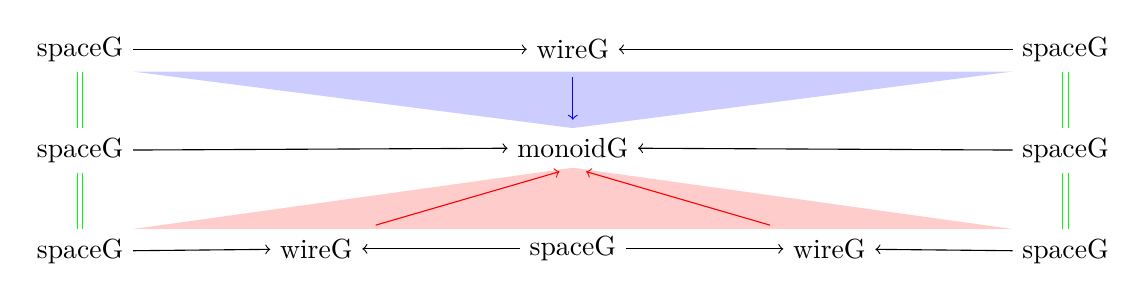
\begin{tikzpicture}
    % r₁
    \node (r1w) {wireG};
    \node[left = 5cm of r1w] (r1l) {spaceG};
    \node[right = 5cm of r1w] (r1r) {spaceG};
    \draw[->] (r1l) -- (r1w);
    \draw[->] (r1r) -- (r1w);
    % s₀
    \node[below = of r1w.center] (m) {monoidG};
    \node[below = of r1l.center] (s0l) {spaceG};
    \node[below = of r1r.center] (s0r) {spaceG};
    \draw[->] (s0l) -- (m);
    \draw[->] (s0r) -- (m);
    % r₀
    \node[below = of s0l.center] (r0ls) {spaceG};
    \node[below = of s0r.center] (r0rs) {spaceG};
    \node[below = of m.center] (r0ms) {spaceG};
    \node[left = 2cm of r0ms] (r0lw) {wireG};
    \node[right = 2cm of r0ms] (r0rw) {wireG};
    \draw[->] (r0ls) -- (r0lw);
    \draw[->] (r0ms) -- (r0lw);
    \draw[->] (r0ms) -- (r0rw);
    \draw[->] (r0rs) -- (r0rw);
    % forward cone
    \fill[fill=red!20] (r0ls.north east) -- (m.south) -- (r0rs.north west);
    % forward rewrite
    \draw[red,->,shorten >=5pt,shorten <=5pt] (r0lw.north east) -- (m.south);
    \draw[red,->,shorten >=5pt,shorten <=5pt] (r0rw.north west) -- (m.south);
    % backward cone
    \fill[fill=blue!20] (r1l.south east) -- (m.north) -- (r1r.south west);
    % backward rewrite
    \draw[blue,->,shorten >=3pt,shorten <=3pt] (r1w) -- (m);
    % equalities between regular heights
    \draw[green,double equal sign distance] (r1l) -- (s0l);
    \draw[green,double equal sign distance] (r1r) -- (s0r);
    \draw[green,double equal sign distance] (r0ls) -- (s0l);
    \draw[green,double equal sign distance] (r0rs) -- (s0r);
  \end{tikzpicture}
\end{document}
